\chapter{DCM for Steady State Responses: Anaesthesia Depth in Rodent Data\label{Chap:data:dcm_ssr}}

\section{Overview}

This chapter describes the analysis of a 2-channel Local Field Potential (LFPs) data set using dynamic causal modelling. The LFPs were recorded from a single rodent using intracranial electrodes \cite{dcm_ssr_anaesthesia}. We thank Marc Tittgemeyer for providing us with this data. The theory behind DCM for steady state responses (DCM-SSR) is described in \cite{dcm_ssr}.

We measured local field potentials from primary (A1) and secondary auditory (A2) cortex in a rodent following the application of four different doses of the anaesthetic agent Isoflurane; 1.4, 1.8, 2.4 and 2.8mg. The rodent was presented with a white noise auditory input for several minutes at each anaesthetised level and time series recordings were obtained for the entire epoch. We performed a steady state DCM analysis using different models, defined according to the extrinsic connections between A1 and A2.

Using Bayesian model comparison we found very strong evidence (Bayes Factor$_{1,2}$ $>$ 100) in favour of a model comprising a network of two neural masses connected by forward (excitatory) and backward (inhibitory + excitatory) connections (\texttt{m1}). This outperformed both a model comprising two neural masses with forward (excitatory) connections only (\texttt{m2}) and a model comprising two neural masses and lateral (inhibitory + excitatory + excitatory) connections only (\texttt{m3}). Within this best performing model we observed changes in forward and backward connections dependent on dose. The strength of inhibitory backward connections increased with successive anaesthetic dose, constituting a greater GABAergic influence postsynaptically for higher doses. Conversely, the solely excitatory forward connections reduced in strength with successive doses

In what follows, these results will be recreated step-by-step using SPM8.

To proceed with the data analysis, first download the data set from the SPM website\footnote{Anaesthesia Depth in Rodent Dataset: \url{http://www.fil.ion.ucl.ac.uk/spm/data/dcm_ssr/}}. The data comprises a data file called \texttt{dLFP\_white\_noise\_r24\_anaes.dat} and its corresponding mat file \texttt{dLFP\_white\_noise\_r24\_anaes.mat}. This has been converted from ASCII data using \texttt{spm\_lfp\_txt2mat\_anaes.m} also on the website and subsequently downsampled to 125 Hz. The conversion script can be altered to suit your own conditions/sampling parameters.

\section{The data}

\begin{itemize}
\item To check data parameters after conversion using ASCII files: in the SPM M/EEG GUI press \textsc{Display/M/EEG}.
\item In our data set we can see there are five trials: four depths of anaesthetic: \texttt{Iso14}, \texttt{Iso18}, \texttt{Iso24} and \texttt{Iso28} and one awake trial \texttt{awake}.
\item We can also see that the data are clean for both the A1 and A2 channels, to view this press \textsc{other}, as the data are LFP type.
\item We are now ready to begin the DCM analysis. To open the DCM GUI press \textsc{DCM} in the SPM M/EEG GUI.
\end{itemize}

\begin{figure}
\begin{center}
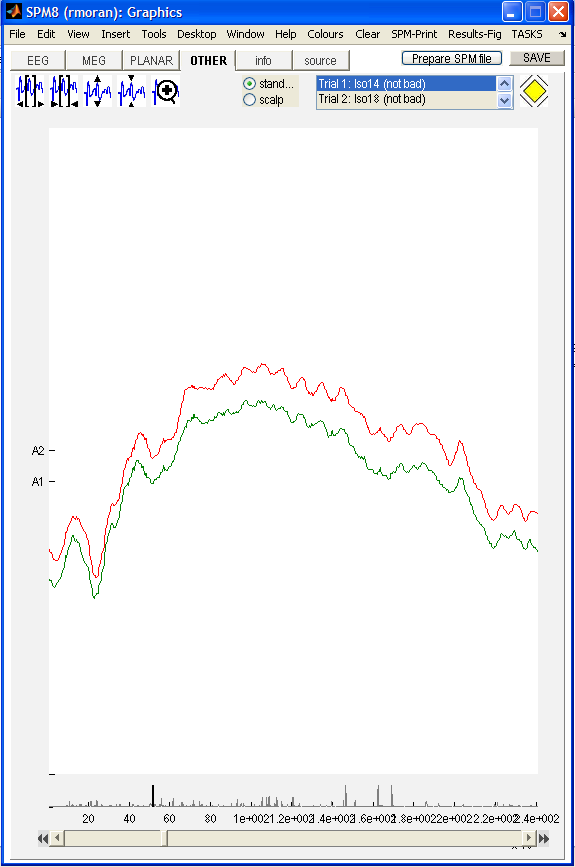
\includegraphics[width=140mm]{dcm_ssr/fig1}
\caption{\em Screenshot of data exploration table. By displaying the converted file \texttt{LFP\_white\_noise\_r24\_anaes.mat} one can check the data quality, length, trials and sampling parameters. \label{dcm_ssr:fig1}}
\end{center}
\end{figure}

\section{Dynamic Causal Modelling of Steady State Responses}

\begin{itemize}
\item Before you begin any DCM analysis you must decide on two things: the data feature from your time series and the model you wish to use.
\item For our long time series we will examine the steady state and so in the top panel of the DCM GUI select \textsc{SSR} in the data drop-down menu.
\item Next in the second drop down menu we select our model. For this LFP data we employ the \textsc{LFP} model and so this is then selected. 
\item Then we are ready to load our data: press \textsc{new data} and select the file \texttt{dLFP\_white\_noise\_r24\_anaes.mat}.
\item Press the red arrow to move forward.
\item The second panel allows you to specify the data and design. We will use the first 30sec of the time series for our analysis. To specify this timing enter \texttt{1} and \texttt{30000} in the time window.
\item Next we select the detrending parameters which we set to \texttt{1} for detrend, \texttt{1} for subsample (as the data has already been downsampled) and \texttt{2} for the modes (in this case this is the same as the number of channels) using the drop down menus.
\item We can then specify which trials we want to use. Since we are interested in the anaesthetized trials we enter \texttt{1 2 3 4} under the trials label and \texttt{effect1 effect2 effect3} in the between trial effects panel. Next we specify the design matrix. This is entered numerically in the large panel. Since we have 4 trials and 3 between trial effects (one less) we enter a matrix with rows:[ 0 1 0 0 ] (row 1), [0 0 1 0] (row 2) and [0 0 0 1] (row 3). This will allow us to examine ``main effect'' differences between the four conditions.\footnote{The effect of anaesthesia could also be specified as a single linear effect, for instance by using a vector of mean-corrected anaesthetic concentrations: [14 18 24 28] - mean([14 18 24 28]) = [-7 -3 3 7]. Here we specified 3 separate effects to show that even when the effects are specified separately, there is a consistent trend in connectivity changes with the increase in anaesthetic concentration.}
\item Press the red arrow to move forward.
\item The third panel contains the spec for the electromagnetic model. This is very simple for LFPs. In the drop down menu select \textsc{LFP}. In the source names panel, enter \texttt{A1} and \texttt{A2}. You are finished.
\item Press the red arrow to move forward.
\item At this point all that is left to specify is the neuronal model. We wish to compare three different models so we can save the specifications so far using the \textsc{save} button and reload the above specs for all three neuronal models.
\item To specify the neuronal model, load the DCM (that you just saved) as it has been so far specified.
\item Our first model is the forward model. So we specify forward connections from A1 to A2 and forward connections from A2 to A1 (Fig~\ref{dcm_ssr:fig2})
\item We also specify the input. In our experiment we assume input at both sources.
\item We finally specify the B effects where we enter our hypothesis of connectivity changes between trial 1 (Iso1.4mg) trial 2 trial 3 and trial 4. Changes will be specified relative to trial 1.
\item We enter the off diagonal entries to correspond to forward connections (as entered in the above panel) and the main diagonal entries to specify intrinsic connectivity changes with A1 and A2 due to (anaesthetic) condition.
\item Finally we enter the frequencies we are interested in: we will fit frequencies from 4 to 48 Hz.
\item To invert the model press \textsc{invert DCM}.
\item Repeat the procedure after loading the saved specs and repeating for new neuronal models as per Fig~\ref{dcm_ssr:fig2}.
\end{itemize}

\begin{figure}
\begin{center}
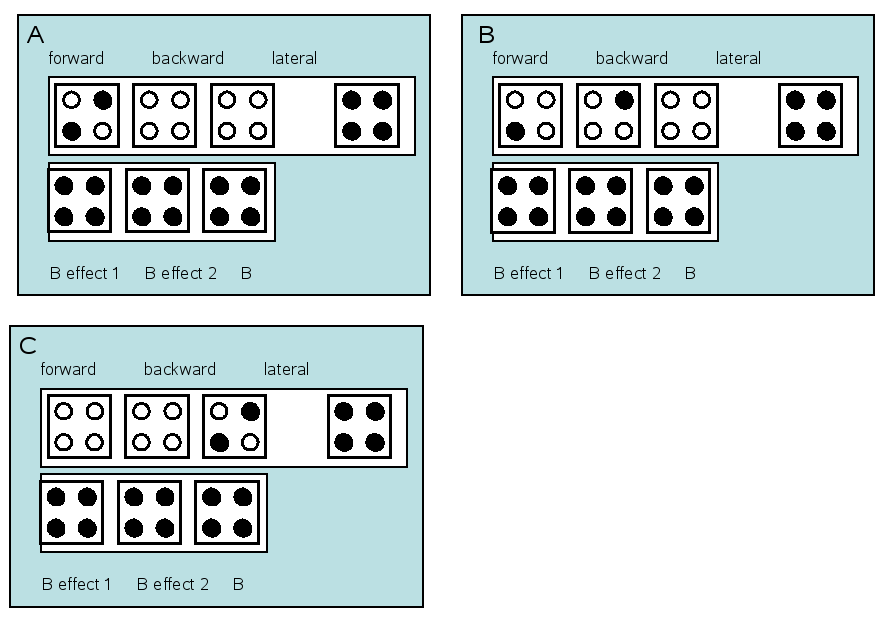
\includegraphics[width=140mm]{dcm_ssr/fig2}
\caption{\em Model Specifications A: forward model, B: forward-backward model, C: lateral model. \label{dcm_ssr:fig2}}
\end{center}
\end{figure}

\section{Results}

\begin{itemize}
\item Once all models have run, we compare their evidences to find to best or winning model.
\item To do this press the \textsc{BMS} button. This will open the SPM batch tool for model selection. Specify a directory to write the output file to.  For the \textsc{Inference method} select \texttt{Fixed effects} (see \cite{klaas_bms} for additional explanations). Then click on \textsc{Data} and in the box below click on \textsc{New: Subject}. Click on \textsc{Subject} and in the box below on \textsc{New: Session}. Click on models and in the selection window that comes up select the DCM mat files for all the models (remember the order in which you select the files as this is necessary for interpreting the results). Then run the model comparison by pressing the green \textsc{Run} button. You will see, at the top, a bar plot of the log-model evidences for all models ~\ref{dcm-ir:fig:6}. At the bottom, you will see the probability, for each model, that it produced the data. By convention, a model can be said to be the best among a selection of other models, with strong evidence, if its log-model evidence exceeds all other log-model evidences by at least 3. You can also compare model evidences manually if you load the DCMs into Matlab's workspace and find the evidence in the structure under \texttt{DCM.F}
\item We can then examine the fits and posterior parameters of the winning model by loading it into the DCM GUI and selecting options from the drop down results menu.
\item In the "trial specific effects" window we are interested particularly in the off-diagonal entries specifying trial specific extrinsic connectivities. Here for the f-b model we see increasing inhibitory (backward) connectivity and decreasing (forward) connectivity for increasing Isoflorane levels (Fig~\ref{dcm_ssr:fig3}. 
\end{itemize}

\begin{figure}
\begin{center}
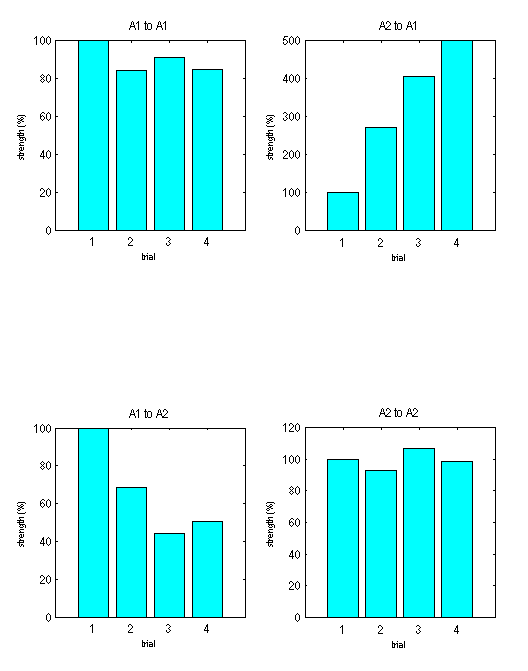
\includegraphics[width=100mm]{dcm_ssr/fig3}
\caption{\em Off diagonal bar charts show forward (A1 to A2) and backward (A2 to A1) connections strengths for trials 1 (1.4 Iso), 2 (1.8 Iso), 3 (2.4 Iso) and 4 (2.8 Iso) \label{dcm_ssr:fig3}}
\end{center}
\end{figure}
